 % !TEX encoding = UTF-8 Unicode

\documentclass[a4paper]{article}

\usepackage{color}
\usepackage{url}
\usepackage[T2A]{fontenc} % enable Cyrillic fonts
\usepackage[utf8]{inputenc} % make weird characters work
\usepackage{graphicx}

\usepackage[english,serbian]{babel}
%\usepackage[english,serbianc]{babel} %ukljuciti babel sa ovim opcijama, umesto gornjim, ukoliko se koristi cirilica

\usepackage[unicode]{hyperref}
\hypersetup{colorlinks,citecolor=green,filecolor=green,linkcolor=blue,urlcolor=blue}

%\newtheorem{primer}{Пример}[section] %ćirilični primer
\newtheorem{primer}{Primer}[section]

\begin{document}

\title{Sajber rat\\ \small{Seminarski rad u okviru kursa\\Racunarstvo i drustvo\\ Matematički fakultet}}

\author{Luka Vukotic\\ mi19120@alas.matf.bg.ac.rs}
\date{24.~maj 2022.}
\maketitle

\abstract{
Dati su odgovori na pitanja kako
definisati sajber rat, kada, kako i zasto se on javlja. Pokazani su neki
(navodni) primeri sajber ratovanja. Predstavljene su neke metode koje se
koriste za napade u sajber prostoru, kao i uzorak heuristickog dijagrama
za klasifikaciju tipova sajber napada. Dati su slikoviti primeri same anatomije i konstrukcije samih sajber napada, kao i razlozi za sve veci broj ljudi koji se bave sajber kriminalom a koji su verovatno ukljuceni u neki vid sajber rata. Takodje, u ovom radu su prikazane i najpopularnije vrste sajber napada kao i neki od nacina njihove prevencije. Pored price o sajber ratu i napadima na globalnom nivou poslednji segment ovog rad je posvecen sajber napadima u Srbiji kao i spremnosti nase drzave da odgovori na ovu sve ucestaliju pojavu.

\tableofcontents

\newpage

\section{Uvod}
\label{sec:uvod}
Sajber rat je potajan i nevidljiv za vecinu. Naime on se odvija u sajber prostoru koga cine sve racunarske mreze na svetu. \textbf{Sajber-prostor} se cesto definise i kao peto ratno podrucje posle kopna, mora, vazduha i svemira za koje si vec znamo.
Termin sajber rata je koriscen u mnogim razlicitim kontekstima, ali u vecini slucajeva sa sobom ne povlaci neki vid nasija na koji smo kroz istoriju navikli kada pomenemo samu rec rat. Sajber rat moze ukljucivati kineticke i nekineticke aktivnosti:
\begin{itemize}
\item Pod pojmom kineticke aktivnosti mislimo na aktivnosti koje se povezuju sa nekim vidom kretanja (npr. pokretanje vojnih snaga, bacanje bombi i koriscenje vojnog naoruzanja u nekom podrucju).
\item Nekineticke aktivnosti su uglavnom usmerene ka bilo kom pristupu suparnickim sajber sistemima, kao sto su prisluskivanje, preuzimanje obavestajnih podataka itd...;
\end{itemize} 

\section{Sta je sajber rat?}
Sto se tice neke univerzalne definicije ona jos uvek ne postoji.
Naime, postoji znacajna debata medju ekspertima u ovoj oblasti o definiciji pojma sajber rata/ratovanja kao i da li tako nesto uopste postoji. Postoji tu dosta problema koji se javljaju prilikom pronalazenja univerzalne definicije.
Prvi problem prilikom definisanja ovog pojma je to sto sajber ratovanje ne ispunjava tipicnu definiciju rata, ali ipak mnoge drzave imaju aktivne sajber operacije za napad i odbranu. Pored vec pomenutih problema, eksponencijalni rast inetrneta i internet tehnologija dovodi do toga da sajber napadi budu sve rasprostranjeniji, i u ovakvom okruzenju uticaj zakona o sajber ratovanju moze biti veoma ogranicen.
Ipak iako ne postoji prihvacena univerzalna definicija postoji vise razlicitih definicija koje mogu biti kandidati:
\begin{itemize}
\item  Talinski prirucnik definise sajber rat kao sajber napad, u
odbranbenoj ili napadnoj sajber operaciji, koji rezultuje u
nasilju, smrti i/ili destrukciji. Nedostatak ove definicije -
iskljucuje npr. sajber operacije dizajnirane da destabilizuju
finansijski sistem nacionalne drzave
\item DCAF odnosno zenevski centar za demokratsku kontrolu oruzanih snaga je usvojio sledecu definiciju: sajber rat je ratno ponasanje koje se sprovodi u virtuelnom svetu koristeci informacije, komunikacionu tehnologiju i mreze, sa namerom da poremeti ili unisti neprijateljske informacione i komunikacione sisteme;


\end{itemize} 




\section{Ucestalost sajber napada}	
\label{sec:termini_i_citiranje}

Sto se tice ucestalosti sajber napada prakticno je nemoguce identifikovati/detektovati svaki sajber napad koji se dogodi.
Neki napadi se mogu neopazeno odvijati godinama (veoma napredan sistem) , drugi su kratkotrajni ali za sobom ne ostavljaju tragove pomocu kojih bi mogli biti otkriveni.
Takodje problem pravi i razvoj same tehnologije jer se sa razvojem povecava broj napada kao i njihova raznovrsnost, ali jedna od dobrih stvari je ta sto se poboljsavaju i odbrambeni mehanizmi kao i sistemi za detekciju napada.  
Deutsche Telekom AG (DTAG), nemacka kompanija za telekomunikacije, uspostavila je mrezu od 97 senzora koji
sluze kao sistem ranog upozorenja koji će u realnom vremenu pruziti  sliku o tekucem sajber napadima. 
Iako je vecina senzora smestena u Nemackoj, DTAG takodje locira honeypots\footnote{Honeypot je racunarski sigurnosni mehanizam postavljen za otkrivanje, uklanjanje ili, na neki nacin, suzbijanje pokusaja neovlasćene upotrebe informacionih sistema.
} 
i senzore u drugim neevropskim zemljama.
\newline
Top petnaest zemalja koje su DTAG senzori zabelezili kao izvor sajber napada istaknuti su na slici 1. 
Otprilike 20\% navedenih sajber napada bilo je poreklom iz Ruske Federacije. 
Prve cetiri navedene drzave, ukljucujuci SAD, Nemacku i Tajvan, cinile su 62\% zastupljenih sajber napada.
Ovi slucajevi pruzaju sliku napada usmerenih na odredjeno geografsko podrucje, u ovom slucaju Evropu.
 


\begin{verbatim}
\end{verbatim}

\begin{figure}[h!]
  \centering
  \begin{center}
  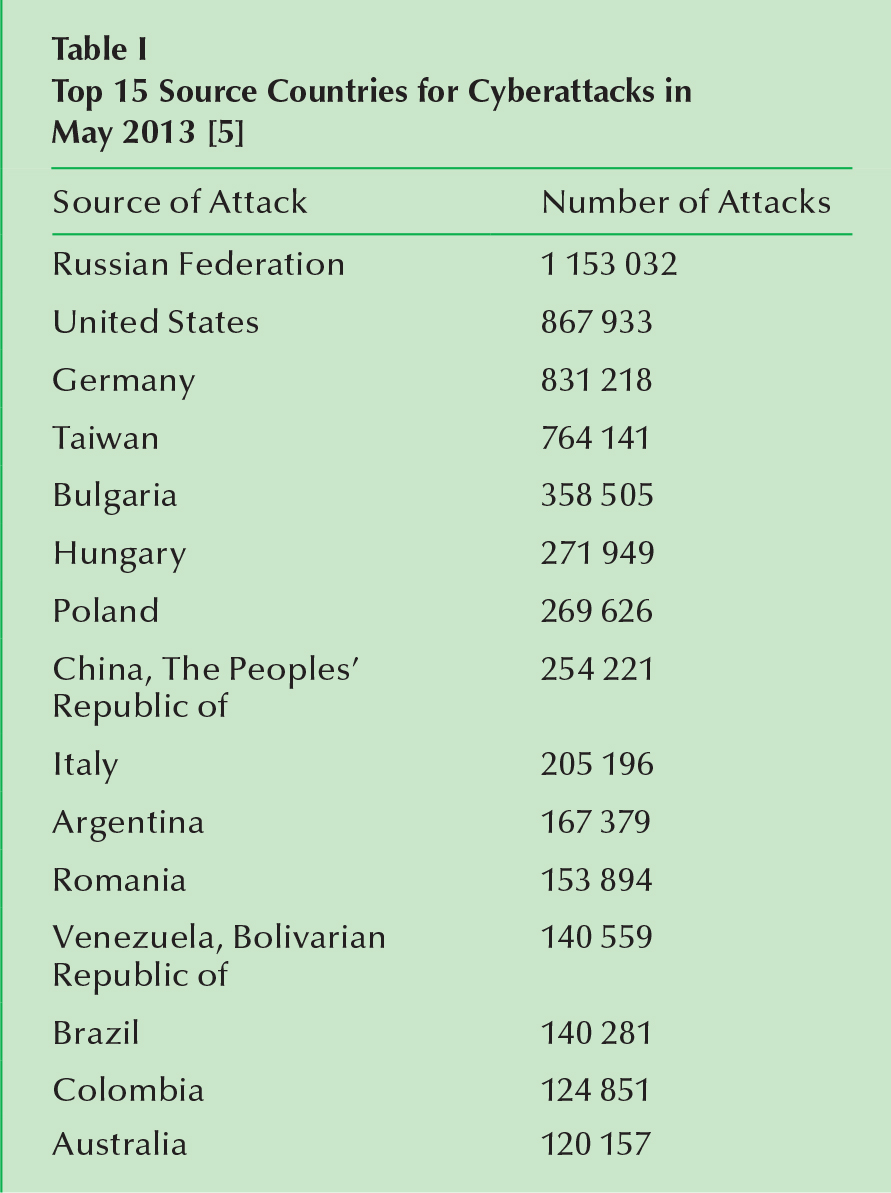
\includegraphics[width=55mm]{slika1.jpg}
  \end{center}
  \caption{Top 15 zemalja izvora za sajber napade u maju 2013. \cite{Overview of current cyber attacks}}
  \label{fig:vr1}
\end{figure}

\newpage

 



\section{Zasto se javlja sajber rat?}
\label{slike_i_tabele}

Za manje drzave ili teroristicke oraganizacije upotreba DDoS (Distributed Denial of Service) napada je mnogo jeftinija (i takodje efikasnija) za pokretanje od konvencionalnih ratnih oruzja i metoda napada protiv naprijatelja, koji uglavnom poseduje veci kolicinu resursa, vojne opreme, vojnih snaga, novca i generalno je veca vojna sila. Samom pojavom sajber rata pojavilo se i novo zanimanje pod nazivom sajber napadac. Sajber napadac za iznajmljivanje je profitabilan posao za one koji su ranije bili samo sajber kriminalci.
Kao sto su primetili mnogi, sajber kriminalci mogu postati sajber ratnici za iznajmljivanje. 
Ovaj lagani prelazak sa sajber kriminalca na sajber ratnika/napadaca sugerise to oslanjanje na strogo razgranicavanje između dve aktivnosti. Nije cesta pojava i da skolovani programeri poneseni novcem i materijalnom dobiti uplivaju u vode sajber kriminala sto cemo kasnije navesti u poglavlju o najpoznatijim zabelezenim sajber napadima. Pored same lakoce napada i kolicine ulozenih resursa prilikom izvodjenja napada, sajber napadi su takodje dosta efikasniji od konvencionalnih/kinetickih napada. Takodje steta koja se napravi prilikom sajber napada kao i prikupljene informacije mogu pomoci i u slucaju same kineticke bitke. Primer za ovako nesto je onesposobljavanje raketne odbrane neke drzave koja je digitalno kontrolisana.
Sajber kriminal i sajber napadi mogu dugorocno dovesti do povecanja sajber napada.
Sami sajber napadi imaju sposobnost da poremete nacin zivota obicnih ljudi (npr. haos koji bi se desio da se izvrsi sajber napad na neki bankomat ili banku i racune u njoj). Takodje medjusobna povezanost globalnih finansijskih institucija povecava rizik za sajber napad.
Ukoliko dodje do napada na neku od finansiskih filijala sirom sveta moguce je preko nje pristupiti zasticenim podacima iz drugih filijala koje su povezane sa hakovanom.







\section{Kako se javlja sajber rat?}
\label{sec:naslov1}

Vecina ljudi je nekada culo za neki od sajber napada koji su se dogodili u Srbiji ili svetu ali celokupna pozadina tog odredjenog dogadjaja je u vecini slucaja tajna ili skrivena. Naime, u vecini slucajeva je pre jednog usepsnog napada vise puta pokusan sajber napad sa istim ciljem ali razlicitim metodama. Kada navodimo sam pojam rata moraju da budu ukljucene dve strane koje se medjusobno sukobljavaju. Veliki broj strucnjaka vec godinama navodi kako se u sajber prostoru, tacnije putem sajber napada sprovodi treci svetski rat (uglavnom navode sukobe Ruske Federacije i Sjedinjenih Americkih Drzava), sto je mozda jos uvek preuvelicano ali samim razvojem tehnologije nema sumnje da ce sajber napadi u buducnosti imati veliku ulogu u svim vecim sukobima kako izmedju drzava tako i izmedju odredjenih korporacija koje jedna drugoj predstavljaju konkurenciju.

Prilikom sajber napada koriste se razni vektori, kako tehnosloski tako i organizacioni. Napadi traze ranjivost u bilo kom od delova koji cine sajber prostor. Istrazivanjima je otkriveno da je veca verovatnoca da ce odredjene vrste napada poteci iz odredjenih drzava i regiona. Na primer 75 procenata dobavljaca internat usluga koji sadrze najvise phishing prevara poticu iz Sjedinjenih Americkih Drzava.

\begin{verbatim}
\end{verbatim}

\begin{figure}[h!]
  \centering
  \begin{center}
  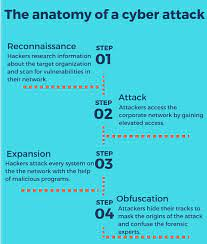
\includegraphics[width=55mm]{index.jpeg}
  \end{center}
  \caption{Slikovito prikazan proces sajber napada}
  \label{fig:vr1}
\end{figure}

\newpage

\section{Metode napada u sajber prostoru}
\label{sec:naslov2}

 \begin{figure}[h!]
  \centering
  \begin{center}
  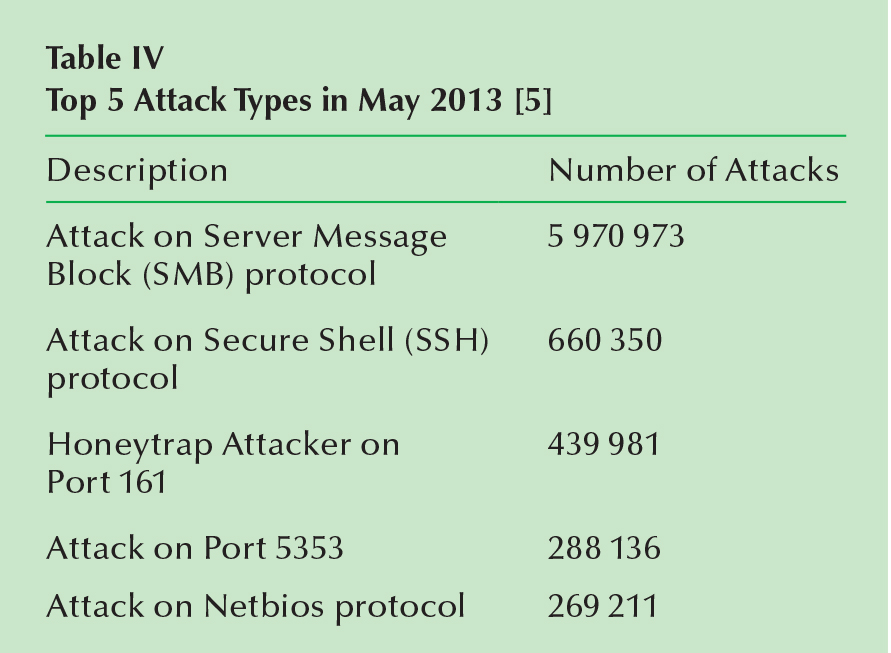
\includegraphics[width=55mm]{slika2.jpg}
  \end{center}
  \caption{Neke od zabelezenih metoda sajber napada}
  \label{fig:vr1}
\end{figure}

Kada pricamo o samim metodama napada u sajber prostoru njih ima neograniceno mnogo, jer se sa razvojem racunarskih tehnologija povecava broj razlicitih nacina samog napada. Veliki uticaj kada pricamo o metodama prilikom izvodjenja sajber napada predstavljaju ciljevi samog sajber napada. Sajber napadi sa kojima se susrecu obicni ljudi u svakodnevnici mogu se nazvati nasumicni napadi. Nasumicni napadi se najcesce desavaju u masovnim kampanjama gde nije targetirana jedna meta, vec se malware plasira ka velikom uzorku meta svih dimenzija, a rezultat je po principu “ ko se upeca – upeca“. Ovakav tip napada primenjuju najcesce distributeri ransomware-a, botnet C&C-a itd gde je sustina u masovnosti, ne u pojedinacnom cilju.
Targetirani napadi su dosta kompleksniji a samim tim zahtevaju i posvecenost napadaca, gde je odvijanje celog napada unapred pripremano, kao i celokupna logistika njemu pridruzena.

Na prikazanoj slici iznad se vidi 5 najpopularnijih vrsta napada otkrivenih u maju 2013te koje je otkrio sistem za identifikaciju napada koji je postavio DTAG. Kao sto se sa slike moze videti vise od 50 procenata ovih napada je na Server Message Block protokolima.
Takodje SCADA sistemi su posebno osetljivi na sajber napade, a time i poprilicno privlacni za sajber napadace. Naime SCADA, ili sistem nadzorne kontrole i prikupljanja podataka se koristi za kontrolu, pracenje i analizu industrijskih uredjaja i procesa.
Sistem se sastoji od softverskih i hardverskih komponenti i omogucava daljinsko prikupljanje podataka kao i prikupljanje na licu mesta. Ovim sistemom se omogucava kompanijama da daljinski upravljaju industrijskim lokacijama kao sto su na primer vetroparkovi itd...
Kako su SCADA sistemi sve vise povezani sa drugim mrezama, ukljucujuci i internet, samo povecavanje sanse za spoljasnju napad se prirodno desava.


\section{Klasifikacija sajber napada}
\label{sec:naslovN}

\begin{figure}[h!]
  \centering
  \begin{center}
  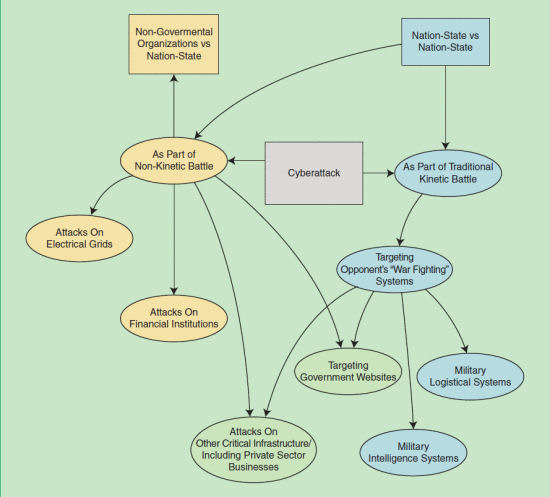
\includegraphics[width=55mm]{proces.jpg}
  \end{center}
  \caption{Proces odvijanja samog napada}
  \label{fig:vr1}
\end{figure}

Sajber napade mozemo podeliti po nivoima pokretanja i nivoima na kojima moze doci do sajber napada:
\begin{itemize}
    \item Vlada naspram vlade (u pogledu kineticke bitke)
    \item Asimetricno ratovanje: nedrzavni akter protiv sopstvenih agencija ili dobavljaca, ili druge vlade (pod nedrzavnim akterom se misli na razne teroristicke grupe, politicke grupe...)
    \item Vlada protiv kriticne infrastrukture druge vlade
    \item  Krivicno nadahnuti hakeri naspram pojedinacnih korisnika;
\end{itemize}

Pored ovakve podele mozemo navesti i razlicite vrste napada po kojima ih mozemo podeliti:
\begin{itemize}
    \item Phishing (pecanje) - napadi ove vrste su izuzetno cesti i ukljucuju slanje velikih kolicina lazne elektronske poste na ime nekog pouzdanog izvora (npr. vasa banka). Elektronske poruke cesto izgledaju kao legitimne, ali povezuju primaoca sa zlonamernom datotekom ili skriptom dizajniranom da omoguci napadacima pristup vasem uredjaju.
    \item MitM ili Man in the Middle - ova vrsta napada se javlja kada napadac presrece dvostranu transkaciju, ubacujuci se u sredinu. Odatle sajber napadaci mogu da kradu podatke i da njima manipulisu tako prekidajuci saobracaj. Ova vrsta napada obicno iskoriscava bezbedonosne propuste u mrezi, ko sto je neobezbedjen javni Wi-Fi, da bi se ubacio izmedju uredjaja posetioca i mreze.
    \item Dos ili Denial of Service - ovi napadi funkcionisu tako sto preplavljuju sisteme, servere ili mreze saobracajem radi preopterecenja resursa i propusnog opega. Rezultat ovog napada je sistem koji nije u stanju da obradi ili ispuni zahteve korisnika.
    Pored DoS postoji i DDoS  ili Distributed Denial of Service. DoS napadi prezasicuju sistemske resurse sa ciljem da ometaju odgovor na zahteve korisnika. Sa druge strane DDoS napad se pokrece sa nekoliko zarazenih host masina sa ciljem da se postigne uskracivanje usluge i da se sistem iskljuci. Ova vrsta napada je pogotovo opasna u slucaju vojnih operacija (npr. potpuno iskljucivanje protivraketnog sistema sto moze dovesti do ozbiljnih posledica).
\end{itemize}    
Pored ovih navedenih postoji jos dosta vrsta kao sto su Malware (zlonamerni softveri), SQL injetion itd...;




\section{Najpoznatiji zabelezeni primeri sajber napada}
\label{sec:naslovM}


Dok je Rusija jos uvek bila u sastavu Sovjetskog saveza 1982. godine, deo njene Trans-sibirskog gasovoda eksplodirao je, navodno zbog implementiranog malvera u piratskoj verziji kanadskog softvera koji je podmetnula CIA. Malver je izazvao malfunkciju u SCADA sistemu koji je pokretao kompletan gasovod.
Hakeri su 2008. godine tokom Gruzijskog rata, odnosno rata u Juznoj Osetiji, obarali Ruske, Osetijske, Gruzijske i Azerbejdzanske sajtove.
Sajber napadi koje su predvodili Rusi:
Postoje tvrdnje da su ruske tajne sluzbe organizivale nekoliko DDoS napada kao deo njihovog sajber ratovanja protiv drugih drzava, najpoznatiji slucajevi su napad na Estoniju 2007. godine, i na Juznu Osetiju, Gruziju i Azerbejdzan 2008. godine. Jedan od identifikovanih hakera rekao je da je bio placen od strane FSB-a da vodi hakerske napade na NATO kompjutere. Studirao je informatiku u Sektoru za odbranu informacija, sto nam pokazuje veoma laku tranziciju u sajber kriminal ljudi koji su skolovani u sektoru informacionih tehnologija.

Iran je bio  zrtva i predator u nekoliko operacija sajber ratovanja. Smatra se vojnom silom u procvatu te je stoga interesantna meta ovakvih napada.
Septembra 2010, Iran je napadnut Staksnet crvom, sa namerom da se specificno pogodi nuklearno postrojenje Natanz. To je bio kompjuterski crv od svega 500 kilobajta koji je zarazio 14 industrijskih sajtova u Iranu, ukljucujuci i Natanz postrojenje. Iako pravi tvorci Staksneta nikada nisu identifikovani, smatra se da su ga razvili napadaci iz SAD-a i Izrael-a i zajedno ga i pustili u pogon. Taj crv je, smatra se, najnapredniji komad malvera ikada otkriven i znacajno je uticao na poimanje opasnosti sajber ratovanja, kao i na razvijanje naprednijih i kvalitetnijih nacina odbrane od ovakvih vrsta napada.

U ratu protiv Hezbolaha 2006 godine, Izrael tvrdi da je doslo do sajber ratovanja tokom sukoba. Obavestajne sluzbe Oruzanih snaga Izraela su dosli do podataka da je nekoliko zemalja na Bliskom istoku unajmilo ruske hakere i naucnike da rade za njih. Kao rezultat toga Izrael je posvetio posebnu paznju sajber taktici i postao time, jedna od retkih drzava u svetu, pored SAD, Francuske i jos nekoliko zemalja, koja se bavi planiranjem za sajber rat. Mnoge medjunarodne IT kompanije se sele i pocinju da istrazuju podrucje Izraela. Ricard Klark dodaje da su "nasi izraelski prijatelji naucili ponesto o programima na kojima mi radimo vec dve decenije" . 
Septembra 2007. godine, Izrael je izvrsio vazdusni napad na Siriju. Namenska industrija SAD-a kao i vojni izvori spekulisu da su izraelci mozda koristili sajber ratovanje kako bi omogucili svojim avionima da prodju neopazano sirijski radar, sto nas vraca na pricu koji smo imali vezanu za opasnost DDoS napada i njihovu vaznost u samim oruzanim sukobima.

\section{Odbrana od sajber napada}

Odbranu od sajber napada u svakodnevnom zivotu mozemo podeliti u tri faze:

1. Faza pre napada
Niko ne moze da zna u kom tacno trenutku ce biti napadnut, ali postoje koraci koji mogu minimizirati takvu mogucnost. Prva i najbitnija stavka vezana za odbranu od sajber napada je edukacija ljudi o samim napadim. Veoma je bitno da ljudi shvate koje sve vrste pretnji postoje i kako na njih da reaguju.
Jedan od primera sve cescih sajber napada je biznis imejl prevara koja je jos poznata kao BEC ili direktorska imejl prevara. Kod ove vrste prevare napadac, pretvarajuci se da je neko od rukovodilaca kompanije (finansijski ili generalni direktor), salje imejl nekom od zaposlenih sa zahtevom da se izvrsi transfer novca ili da mu posalje lozinku. Primalac ovakve poruke mora da bude oprezan i da proveri da li u takvom zahtevu ima neceg neuobicajenog. Na primer, da li je ton u kome je napisan imejl neuobicajeno formalan ili pak previse neformalan? Da li je nesto drugacije kada je u pitanju font ili odvajanje reci/recenica? Ako jeste, primalac bi trebalo da detaljnije pogleda imejl adresu. Mozda na prvi pogled izgleda isto, ali kada se obrati paznja moguce je da je neko slovo zamenjeno ili potpuno drugacije.

2. Faza u toku napada
Jedna od najgorih stvari koje mogu da nas zadese je da nas sajber napad uhvati nespremne. Najboji nacin da se ublaze posledice sajber napada je da postoji detaljan i dobro uvezban plan reagovanja u slucaju incidenta koji se momentalno moze pokrenuti. Plan bi trebalo da sadrzi vise detalja, ukljucujuci i informacije o tome koga kontaktirati. Bitno je da napad prijavite nadleznim drzavnim organima. U Srbiji se sajber napadi prijavljuju Odeljenju za visokotehnoloski kriminal, odnosno policiji koja takve prijave salje pomenutom odeljenju. Takodje, jako bitna stvar je da obavestite ljude u svojoj okolini da se paze stvari koje su se vama dogodile kako bi se sledeci put prepoznao napad na vreme. Mozda sve ovo zvuci kao previse posla, i verovatno vecina ljudi nema previse vremena da se bavi ovakvim stvarima ali je najbitnije postojanje svesti o samoj mogucnosti napada.

3. Faza nakon napada
Ukoliko dodje do napada morate pozvati ljude koji su strucni u ovoj oblasti koji moraju da otkriju na koji nacin se tacno napad odvijao. Da li je do napada doslo zbog lose konfiguracije web servera? Nisu uradjene zakrpe za Windows radne stanice? Web proxy podesavanja daju previse ovlascenja? Identifikujte izvor kako bi sprecili da ponovo budete napadnuti na isti nacin. U suprotnom, naci cete se u zacaranom krugu stalnog ciscenja i ponovnih infekcija (ove stvari su pogotovo bitne za kompanije i zaposlene u njima). Potrebno je da razumete ranjivosti koje su napadaci eksploatisali, i potruditi se da u buduce preduzmete sve odbrambene mere.

\section{Sajber napadi u Srbiji}

Srbija se u junu 2021. godine nasla na sedmom mestu globalne liste zemalja po broju napada na industrijske racunare, prema podacima kompanije "Kaspersky". Prema podacima RATEL-a na svakih 39 sekundi desi jedan sajber napad u nasoj zemlji.
Problemi u vezi sa hakerskim napadima sve su cesci kako u svetu, tako i u Srbiji, zato sto postajemo sve zavisniji od tehnologije. Naime, sto je jedna drzava razvijenija i sto vise koristi naprednu tehnologiju postaje ranjivija i ugrozenija od sajber napada.
Eksperti za ovu oblast navode da je jedan od glavnih problema slab mehanizam odbrane, ali  oni dodaju da napredak u Srbiji postoji. 
Istrazivanje koje je sprovedeno u 69 gradova i opstina u Srbiji pokazuje da 58 posto lokalnih samouprava nije proveravalo bezbednost mreze, a niko od anketiranih nije u poslednjih godinu dana testirala plan oporavka u slucaju kolapsa sistema. Dok takodje postoji podatak da 47\% lokalnih samopurava bilo meta sajber napada, a 12\% ni ne zna da su bili napadnuti.  

\addcontentsline{toc}{section}{Literatura}
\appendix

\iffalse
\bibliography{seminarski} 
\bibliographystyle{plain}
\fi

\begin{thebibliography}{9}

\bibitem{Cyberwar} Angelyn Flowers, Sherali Zeadally, Cyberwar: The What, When, Why, and How
  Article in IEEE Technology and Society Magazine · September 2014,
  https://technologyandsociety.org/cyberwar-the-what-when-why-and-how/

\bibitem{DCAF Horizons} F. Schreier, On Cyberwarfare: DCAF Horizons 2015 Working
Paper. Geneva: Defense Center for Armed Forces, 2013.

\bibitem{Cyberwar thresholds and effects} J. Lewis, “Cyberwar thresholds and effects,” IEEE Security and
Privacy, pp. 23–29, Sept./Oct. 2011.

\bibitem{Declarations of cyberwar} W. Jones, “Declarations of cyberwar: What the revelations about
the U.S.-Israeli origin of Stuxnet mean for warfare,” IEEE Spectrum,
pp. 18, Aug. 2012

\bibitem{Overview of current cyber attacks}Deutsche Telekom AG, “Overview of current cyber attacks;” http://
www.sicherheitstacho.eu/, accessed June 6, 2013.

\bibitem{The Threat in Cyberspace} R. O’Harrow, Jr., Zero Day: The Threat in Cyberspace. New York,
NY: Diversion Books, Washington Post E-Book, 2013.

\bibitem{Improving critical infrastructure cybersecurity}B. Obama, “Executive order 13636: Improving critical infrastruc-
ture cybersecurity,” Federal Register, vol. 78, no. 33, part III, Feb.19,
2013.

\bibitem {Cyber war}Sajber rat Wikipedia

\bibitem {Sajber napadi u Srbiji}https://www.euronews.rs/srbija/drustvo/25537/jedan-sajber-napad-na-svakih-39-sekundi-srbija-u-vrhu-po-broju-hakerskih-upada/vest


\end{thebibliography}

\end{document}
